
\section{Thursday}\index{week7_Thursday_lecture}

Three ways for matrix decomposition are significant in linear alegbra:
\[
\left\{
\begin{lgathered}
\text{LU (from \emph{Gaussian elimination})}\\
\text{QR (from \emph{Orthogonalization})}\\
\text{SVD (from \emph{eigenvalues and eigenvectors})}
\end{lgathered}
\right.
\]
We have learnt the first two decomposition. And the third way is increasingly significant in the information age.

In the last lecture we learnt that any real symmetric matrix adimits \textit{diagonalization}, i.e., \textit{eigendecomposition}. However, can we get some \emph{universal} decomposition, i.e., Is there any decomposition that can be applied to all matrices?

The anwer is yes. The key idea behind is to do \textit{symmetrization}. We have to consider $\bm A\bm A\trans$ and $\bm A\trans\bm A$.
\subsection{SVD: Singular Value Decomposition}
\begin{theorem}[SVD]
Given any matrix $\bm A\in\mathbb{R}^{m\times n}$, there exists a 3-tuple $(\bm U,\bm\Sigma,\bm V)\in\mathbb{R}^{m\times m}\times \mathbb{R}^{m\times n}\times \mathbb{R}^{n\times n}$ such that
\[
\bm A=\bm U\bm\Sigma\bm V\trans,
\]
where $\bm U,\bm V$ are \emph{orthogonal}, and $\bm\Sigma$ takes the form
\[
\bm\Sigma_{ij}=\left\{
\begin{aligned}
\sigma_i,&\quad i=j\\
0,&\quad i\ne j
\end{aligned},
\right.
\]
with $\sigma_1\ge\sigma_2\ge\cdots\ge\sigma_p\ge0$ and with $p=\min\{m,n\}$.
\end{theorem}
\begin{remark}
\begin{itemize}
\item
If $\bm V=\bm U$, this decomposition is exactly \emph{eigen-decomposition}.
\item
Specifically speaking,
\begin{itemize}
\item
$\bm U\in\mathbb{R}^{m\times m}$ such that its columns are eigenvectors of $\bm A\bm A\trans$
\item
 $\bm V\in\mathbb{R}^{n\times n}$ such that its columns are eigenvectors of $\bm A\trans\bm A$
 \item
$\bm\Sigma\in\mathbb{R}^{m\times n}$ looks like a diagonal matrix, i.e., it has the form
\[
\begin{array}{ll}
\bm\Sigma=\begin{pmatrix}
\sigma_1&&\\&\ddots&\\&&\sigma_n\\
0&\dots&0\\\vdots&\ddots&\vdots\\0&\dots&0
\end{pmatrix}\text{ if $m\ge n$}\\
\bm\Sigma=\begin{pmatrix}
\sigma_1&&&0&\dots&0\\&\ddots&&\vdots&\ddots&\vdots\\&&\sigma_m&0&\dots&0\end{pmatrix}\text{ if $m< n$}.
\end{array}
\]
\end{itemize}
with $\sigma_i=\sqrt{\lambda_i}$ for $i=1,2,\dots,\min\{m,n\}$, where \textit{$\lambda_i$'s are eigenvalues of $\bm A\bm A\trans$ (if $m< n$) or $\bm A\trans\bm A$. (if $m\ge n$)})
\end{itemize}
\begin{definition}[SVD]
The above decomposition is called the \emph{singular value decomposition (SVD)}
\begin{itemize}
\item
$\sigma_i$ is called the $i$th \emph{singular value}
\item
The columns of $\bm U$ and $\bm V$, $\bm u_i$ and $\bm v_i$ are called the $i$th \emph{left and right singular vectors}, respectively.
\item
$(\sigma_i,\bm u_i)$ are the eigen-pairs of $\bm A\bm A\trans$; $(\sigma_i,\bm v_i)$ are the eigen-pairs of $\bm A\trans\bm A$ for $i=1,2,\dots,\min\{m,n\}$.
\item
The following notations may be used to denote the singular values of $\bm A$:
\[
\sigma_{\max}(\bm A)\ge\sigma_1(\bm A)\ge\sigma_2(\bm A)\ge\cdots\ge\sigma_p(\bm A)=\sigma_{\min}(\bm A)
\]
\end{itemize}
\end{definition}
\end{remark}
The proof for the SVD decomposition is constructive. To see the insights of the proof, let's study the case $m=n$ first, then we extend the proof for general case:
\begin{proposition}
SVD always exists for any \emph{real square nonsingular} matrix.
\end{proposition}
\begin{proof}
For $\bm A\in\mathbb{R}^{n\times n}$, you may verify that $\bm A\bm A\trans$ is PD, thus it admits the eigen-decomposition:
\begin{equation}
\begin{array}{ll}
\bm A\bm A\trans=\bm U\bm\Sigma\bm U\trans,
&
\mbox{with }\lambda_1\ge\cdots\ge\lambda_n>0.
\end{array}
\end{equation}

We define $\bm\Sigma:=\diag(\sqrt{\lambda_1},\dots,\sqrt{\lambda_m})$ and $\bm V:=\bm A\trans\bm U\bm\Sigma^{-1}$.

You may verify that $\bm U\bm\Sigma\bm V\trans=\bm A$ and $\bm V\trans\bm V=\bm I$, i.e., $\bm V$ is orthogonal. The proof is complete.
\end{proof}
\begin{proposition}
SVD always exists for any \emph{real} matrix.
\end{proposition}
\begin{proof}
\begin{itemize}
\item
Firstly, consider the matrix product $\bm A\bm A\trans$. Since $\bm A\bm A\trans\in\mathbb{S}^m$ and $\bm A\succeq0$, we can decompose $\bm A\bm A\trans$ as
\begin{equation}\label{Eq:8:9}
\bm A\bm A\trans=\bm U\bm\Sigma\bm U\trans
=\begin{bmatrix}
\bm U_1&\bm U_2
\end{bmatrix}
\begin{bmatrix}
\tilde{\bm\Sigma}&\bm0\\\bm0&\bm0
\end{bmatrix}
\begin{bmatrix}
\bm U_1\trans&\bm U_2\trans
\end{bmatrix}=\bm U_1\tilde{\bm\Sigma}\bm U_1\trans
\end{equation}
where:
\begin{itemize}
\item
we assume that the eigenvalues are ordered, i.e., 
\[
\begin{array}{lll}
\lambda_1\ge\dots\ge\lambda_r>0,
&
\mbox{and}
&
\lambda_{r+1}=\cdots=\lambda_p=0
\end{array}
\]
with $r$ being the number of nonzero eigenvalues
\item
$\bm U\in\mathbb{R}^{m\times m}$ denotes an orthogonal matrix, and its columns are the corresponding eigenvectors
\item
We partition $\bm U$ as
\[
\begin{array}{ll}
\bm U=\begin{bmatrix}
\bm U_1&\bm U_2
\end{bmatrix},
&
\bm U_1\in\mathbb{R}^{m\times r},\bm U_2\in\mathbb{R}^{m\times (m-r)},
\end{array}
\]
and $\tilde{\bm\Sigma}=\diag(\lambda_1,\dots,\lambda_r)$.
\end{itemize}
\item
Secondly, we show that 
\begin{equation}\label{Eq:8:12}
\bm U_2\trans\bm A=0
\end{equation}

Since $\bm U$ is orthogonal, we obtain:
\[
\bm U\trans\bm U=\begin{bmatrix}
\bm U_1\trans\\\bm U_2\trans
\end{bmatrix}\begin{bmatrix}
\bm U_1&\bm U_2
\end{bmatrix}=\begin{bmatrix}
\bm U_1\trans\bm U_1&\bm U_1\trans\bm U_2\\
\bm U_2\trans\bm U_1&\bm U_2\trans\bm U_2
\end{bmatrix}=\bm I\implies
\bm U_2\trans\bm U_1=\bm0.
\]
Substituting Eq.(\ref{Eq:8:9}) into $\bm U_2\trans\bm A(\bm U_2\trans\bm A)\trans$, we obtain:
\begin{equation}
\bm U_2\trans\bm A(\bm U_2\trans\bm A)\trans
=(\bm U_2\trans\bm U_1)\tilde{\bm\Sigma}\bm U_1\trans\bm U_2=\bm0\label{Eq:8:10}
\end{equation}
By Eq.(\ref{Eq:8:10}) and the simple result that $\bm B\bm B\trans=\bm0$ implies $\bm B=\bm0$ (write $\bm B$ into column vectors form to verify it), we conclude that $\bm U_2\bm A=\bm0$
\item
Thirdly, we construct the following matrices:
\[
\begin{array}{ll}
\widehat{\bm\Sigma}=\tilde{\Sigma}^{1/2}=\diag(\sqrt{\lambda_1},\dots,\sqrt{\lambda_r}),
&
\bm V_1=\bm A\trans\bm U_1\widehat{\bm\Sigma}^{-1}\in\mathbb{R}^{n\times r}.
\end{array}
\]
Combining it with Eq.(\ref{Eq:8:9}), we can verify that $\bm V_1\trans\bm V_1=\bm I$. Furthermore, there exists a matrix $\bm V_2\in\mathbb{R}^{n\times (n-r)}$ such that $\bm V=\begin{bmatrix}
\bm V_1&\bm V_2
\end{bmatrix}$ is orthogonal. Moreover, we can verify that
\begin{equation}\label{Eq:8:11}
\begin{array}{ll}
\bm U_1\trans\bm A\bm V_1=\widehat{\bm\Sigma},
&
\bm U_1\trans\bm A\bm V_2=\bm0
\end{array}
\end{equation}
\item
Fourthly, consider the matrix product $\bm U\trans\bm A\bm V$. From Eq.(\ref{Eq:8:11}) and Eq.(\ref{Eq:8:12}), we have
\begin{align*}
\bm U\trans\bm A\bm V&=\begin{bmatrix}
\bm U_1\trans\bm A\bm V_1&
\bm U_1\trans\bm A\bm V_2
\\
\bm U_2\trans\bm A\bm V_1
&
\bm U_2\trans\bm A\bm V_2
\end{bmatrix}\\&=\begin{bmatrix}
\widehat{\bm\Sigma}&\bm0\\\bm0&\bm0
\end{bmatrix}:=\bm\Sigma
\end{align*}
By multiplying the above equation on the left by $\bm U$ and on the
right by $\bm V\trans$, we obtain the desired result $A = \bm U\bm\Sigma\bm V\trans.$ The proof is complete.
\end{itemize}
\end{proof}

\subsection{Remark on SVD decomposition}
\subsubsection{Remark 1: Different Ways of Writing out SVD}
\begin{definition}[Paritioned form of SVD]
let $r$ be the number of nonzero singular values, and note that $\sigma_1\ge\cdots\ge\sigma_r>0, \sigma_{r+1}=\cdots=\sigma_p=0$. Then from the standard form, we derive the \emph{partitioned form of SVD}:
\begin{equation}\label{Eq:8:13}
\bm A=\begin{bmatrix}
\bm U_1&\bm U_2
\end{bmatrix}\begin{bmatrix}
\tilde{\bm\Sigma}&\bm0\\\bm0&\bm0
\end{bmatrix}\begin{bmatrix}
\bm V_1\trans\\\bm V_2\trans
\end{bmatrix}
\end{equation}
where:
\begin{itemize}
\item
$\tilde{\bm\Sigma} = \diag(\sigma_1,\dots,\sigma_r)$
\item
$\bm U_1=\begin{bmatrix}
\bm u_1&\cdots&\bm u_r
\end{bmatrix}\in\mathbb{R}^{m\times r}, \bm U_2=\begin{bmatrix}
\bm u_{r+1}&\cdots&\bm u_m
\end{bmatrix}\in\mathbb{R}^{m\times (m-r)}$
\item
$\bm V_1=\begin{bmatrix}
\bm v_1&\cdots&\bm v_r
\end{bmatrix}\in\mathbb{R}^{n\times r}, \bm V_2=\begin{bmatrix}
\bm v_{r+1}&\cdots&\bm v_n
\end{bmatrix}\in\mathbb{R}^{n\times (n-r)}$
\end{itemize}
Note that $\bm U_1,\bm U_2,\bm V_1,\bm V_2$ are semi-orthogonal, i.e., they all have orthonormal columns.
\end{definition}
\begin{definition}[Thin SVD]
We can re-write Eq.(\ref{Eq:8:13}) as the \emph{thin form of SVD}:
\begin{equation}\label{Eq:8:14}
\bm A=\bm U_1\tilde{\bm\Sigma}\bm V_1\trans
\end{equation}
\end{definition}
\begin{definition}[Outer-product form]
By expanding the Eq.(\ref{Eq:8:14}), we derive the \emph{outer-product form of SVD}:
\begin{equation}\label{Eq:8:15}
\bm A=\sum_{i=1}^p\sigma_i\bm u_i\bm v_i\trans
=\sum_{i=1}^r\sigma_i\bm u_i\bm v_i\trans
\end{equation}
\end{definition}

\subsubsection{Remark 2: SVD and Eigen-decomposition}
The eigenvalues for $\bm A\trans\bm A$ and $\bm A\bm A\trans$ are the same for first $p$ terms.
\begin{proposition}
Suppose $\bm A$ admits the SVD $\bm A=\bm U\bm\Sigma\bm V\trans$, then we have:
\begin{align}
\bm A\bm A\trans&=\bm U\bm D_1\bm U\trans,\qquad
\bm D_1=\bm\Sigma\bm\Sigma\trans=\diag(\sigma_1^2,\dots,\sigma_p^2,\underbrace{0,\dots,0}_{\text{$m-p$ zeros}})\\
\bm A\trans\bm A&=\bm V\bm D_2\bm V\trans,\qquad
\bm D_2=\bm\Sigma\trans\bm\Sigma=\diag(\sigma_1^2,\dots,\sigma_p^2,\underbrace{0,\dots,0}_{\text{$n-p$ zeros}})
\end{align}
\end{proposition}
\begin{proof}
Just apply the SVD form and the orthogonality of $\bm U$ and $\bm V$.
\end{proof}

\subsubsection{Remark 3: SVD and Subspace}
We are curious about how many singular values of $\bm A$ are nonzero.
\begin{proposition}\label{Prop:8:5}
The following properties hold:
\begin{enumerate}
\item
$\mathcal{C}(\bm A)=\mathcal{C}(\bm U_1), \mathcal{C}(\bm A)^\perp=\mathcal{C}(\bm U_2)$;
\item
$\mathcal{C}(\bm A\trans)=\mathcal{C}(\bm V_1), \mathcal{C}(\bm A\trans)^\perp=\mathcal{N}(\bm A)=\mathcal{C}(\bm V_2)$;
\item
$\rank(\bm A)=r$, i.e., the number of nonzero singular values.
\end{enumerate}
\end{proposition}
\begin{proof}
The above properties are easily seen to be true using SVD. Also, you should apply the definition for column space and null space. You should verify these properties by yourself. 
\begin{subequations}
\begin{equation}
\mathcal{C}(\bm A)=\{\bm y\in\mathbb{R}^m\mid\bm y=\bm{Ax}, \bm x\in\mathbb{R}^n\}
\end{equation}
\begin{equation}
\mathcal{N}(\bm A)=\{\bm x\in\mathbb{R}^n\mid \bm{Ax}=\bm0\}
\end{equation}
\end{subequations}
For the third part of proposition(\ref{Prop:8:5}), since $\rank(\bm A)=\dim(\mathcal{C}(\bm A))=\dim(\mathcal{C}(\bm U_1))$, and $\bm U_1$ has $r$ orthonormal columns, we derive that $\dim(\mathcal{C}(\bm U_1))=r=\rank(\bm A).$
\end{proof}

For the SVD decomposition
\[
\bm A=\bm U\bm\Sigma\bm V\trans,
\]
we can convert it into the following two forms:
\begin{gather*}
\bm A\bm V=\bm U\bm\Sigma\bm V\trans\bm V=\bm U\bm\Sigma\\
\bm A=\bm U\bm\Sigma\bm V\trans\implies
\bm A\trans=\bm V\bm\Sigma\bm U\trans\implies
\bm A\trans\bm U=\bm V\bm\Sigma\bm U\trans\bm U=\bm V\bm\Sigma.
\end{gather*}
If we write it into vector forms, we obtain:
\begin{equation}
\left\{
\begin{aligned}
\bm A\bm v_j=\sigma_j\bm u_j\\
\bm A\trans\bm u_j=\sigma_j\bm v_j
\end{aligned}
\right.,\quad j=1,2,\dots,r.\label{Eq:8:19}
\end{equation}
The columns of $\bm U$ ($\bm u_j$) are called the \emph{left singular vector} of $\bm A$; the columns of $\bm V$ ($\bm v_j$) are called the \emph{right singular vector} of $\bm A$; $\sigma_j$ is called the \emph{singular value}.

We can easily understand the proposition(\ref{Prop:8:5}) and Eq.(\ref{Eq:8:19}) by the following graph:
\begin{figure}[H]
\centering
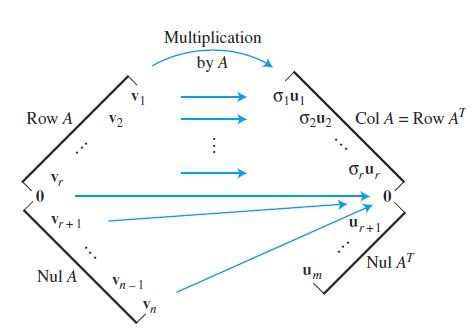
\includegraphics[width=10cm]{week7/fundamental}
\caption{The fundamental spaces and the action of $\bm A$.}
\end{figure}
\textbf{Explanation:}
\begin{itemize}
\item
When $\{\bm v_1,\dots,\bm v_r\}$ are multiplied by $\bm A$, they are converted into $\{\sigma_1\bm u_1,\dots,\sigma_r\bm u_r\}$; when $\{\bm v_{r+1},\dots,\bm v_{n}\}$ are multiplied by $\bm A$, they are converted into $\bm0$.
\item
The first $r$ columns of $\bm V$ forms the basis for the row space of $\bm A$, i.e., $\mathcal{C}(\bm V_1)=\mathcal{C}(\bm A\trans)$.
\item
The last $n-r$ columns of $\bm V$ forms the basis for the null space of $\bm A$, i.e., $\mathcal{C}(\bm V_2)=\mathcal{N}(\bm A)$.
\item
The first $r$ columns of $\bm U$ forms the basis for the column space of $\bm A$, i.e., $\mathcal{C}(\bm U_1)=\mathcal{C}(\bm A)$.
\item
The last $m-r$ columns of $\bm U$ forms the basis for the null space of $\bm A\trans$, i.e., $\mathcal{C}(\bm U_2)=\mathcal{N}(\bm A\trans)$
\end{itemize}

Recall the outer-product form of SVD, 
\[
\bm A=\sigma_1\bm u_1\bm v_1\trans+\dots+\sigma_r\bm u_r\bm v_r\trans
\]
where $r=\rank(\bm A)=\text{number of nonzero singular values,}$ which is the third meaning for the rank:
\begin{remark}
Up till now, $\rank(\bm A)$ has three meanings:
\begin{itemize}
\item
$\rank(\bm A)=\dim(\row(\bm A))$
\item
$\rank(\bm A)=\dim(\col(\bm A))$
\item
$\rank(\bm A)=$ number of nonzero singular values of $\bm A$.
\end{itemize}
\end{remark}


\begin{remark}
However, $\rank(\bm A)\ne$ number of nonzero eigenvalues. Let me raise a counterexample:
\[
\bm A=\begin{bmatrix}
0&1\\0&0
\end{bmatrix}
\]
then eigenvalues are $\lambda_1=\lambda_2=0$, and $\rank(\bm A)=1.$
\end{remark}
\begin{remark}
Also, note that many properties can be easily proved by \emph{thin} or \emph{outer-product} form of	SVD. For example, $\rank(\bm A\trans\bm A)=\rank(\bm A)$. If you have no ideas of a proof in exam, you may try SVD.
\end{remark}




\subsubsection{Compact SVD}
Due to the outer-product form of SVD, i.e., any matrix with rank $r$ can be factorized into
\begin{align*}
\bm A&=\bm U\bm\Sigma\bm V\trans\\
&=\begin{bmatrix}
\bm u_1&\dots&\bm u_r
\end{bmatrix}\begin{pmatrix}
\sigma_1&&\\&\ddots&\\&&\sigma_r
\end{pmatrix}\begin{bmatrix}
\bm v_1\trans\\\vdots\\\bm v_r\trans
\end{bmatrix},
\end{align*}
we obtain the following corollary:
\begin{corollary}
Every rank $r$ matrix can be written as the sum of $r$ rank $1$ matrices. Moreover, these matrices could be perpendicular!
\end{corollary}
What's the meaning of perpendicular?
\begin{definition}[perpendicular for matrix]
For two real $n\x n$ matrix $\bm A$ and $\bm B$, they are said to be \emph{perpendicular} (\emph{orthogonal}) if the inner product between $\bm A$ and $\bm B$ is zero:
\[
\inp{\bm A}{\bm B}=\trace(\bm B\trans\bm A)=\sum_{i,j=1}^{n}\bm A_{ij}B_{ij}=0.
\]
\end{definition}
Decompose $\bm A:=\sum_{i=1}^{r}\sigma_i\bm u_i\bm v_i\trans$. If we set $\bm A_i=\bm u_i\bm v_i\trans\sigma_i$, let's show $\bm A_i$'s are perpendicular:
\begin{align*}
\inp{\bm A_i}{\bm A_j}&=\trace(\bm A_j\trans\bm A_i)\\
&=\trace(\sigma_i\sigma_j\bm v_j\bm u_j\trans\bm u_i\bm v_i\trans)=\sigma_i\sigma_j\trace(\bm v_j\bm u_j\trans\bm u_i\bm v_i\trans)\\
&=\sigma_i\sigma_j\trace(\bm v_j(\bm u_j\trans\bm u_i)\bm v_i\trans)=\sigma_i\sigma_j\trace(\bm v_j\bm 0\bm v_i\trans)\\
&=0.
\end{align*}

How many rank 1 matrices do we need to pick to construct matrix $\bm A$? In fact, this number has no upper bound. For example, if we obtain
\[
\bm A=\bm u_1\bm v_1\trans+\bm u_2\bm v_2\trans
\]
Then we can always decompose any rank 1 matrix into 2 rank 1 matrices:
\[
\bm A=\bm u_1\bm v_1\trans+\frac{1}{2}\bm u_2\bm v_2\trans+\frac{1}{2}\bm u_2\bm v_2\trans.
\]
But this number has a lower bound, that is rank. In other words, $\rank(\bm A)$ = smallest number of rank 1 matrices with sum $\bm A$.

\subsection{Best Low-Rank Approximation}
Given matrix $\bm A$. What is the \textit{best rank $k$ approximation}? In other words, given matrix $\bm A\in\mathbb{R}^{m\x n}$, what is the optimal solution for the optimization:
\begin{align*}
  \min_{\bm Z}\quad        & \|\bm A-\bm Z\|^2_{F} \\
  \text{s.t.\quad} &  \rank(\bm Z)=k &     \\
                   &\bm Z\in\mathbb{R}^{m\x n}
\end{align*}
Firstly let's introduce the definition for Frobenius norm:
\begin{definition}[Frobenius norm]
The Frobenius norm for $m\x n$ matrix $\bm A$ is given by
\[
\|\bm A\|_{F}=\sqrt{\inp{\bm A}{\bm A}}=\sqrt{\trace(\bm A\trans\bm A)}.
\]
\end{definition}
\begin{theorem}\label{proposition_8.4}
Suppose the SVD for $\bm A\in\mathbb{R}^{m\x n}$ is given by
\[
\bm A=\sigma_1\bm u_1\bm v_1\trans+\dots+\sigma_r\bm u_r\bm v_r\trans.
\]
with $\sigma_1\ge\sigma_2\ge\dots\ge0$.

Then the best rank $k$($k\le r$) approximation of $\bm A$ is
\[
\bm A_k=\sigma_1\bm u_1\bm v_1\trans+\dots+\sigma_k\bm u_k\bm v_k\trans.
\]
\end{theorem}
For example, $\sigma_1\bm u_1\bm v_1\trans$ is the best rank 1 approximation of $\bm A$.
\subsubsection{Analogy with least square problem}
For least squares problem, the key is to do approximation for $\bm b\in\mathbb{R}^m$. In other words, we just do a projection from $\bm b$ to the plane $\{\bm{Ax}|\bm x\in\mathbb{R}^n\}$:
\begin{figure}[H]
\centering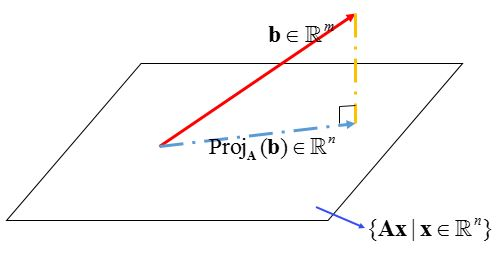
\includegraphics{week7/least_square}
\caption{Least square problem: find $\bm x$ such that $\bm{Ax}=\Proj_{\mathcal{C}(\bm A)}(\bm b).$}
\end{figure}
\begin{remark}
For the least squares problem
\begin{align*}
  \min_{\bm x}\quad        & \|\bm A\bm x-\bm b\|^2 \\
  \text{s.t.\quad} &  \bm x\in\mathbb{R}^{n}
\end{align*}
with $\bm A\in\mathbb{R}^{m\times n}$ and $\bm b\in\mathbb{R}^m$, the key is to do the projection of $\bm b$ onto $\mathcal{C}(\bm A)$, thus it suffices to solve the \emph{equality}
\[
\bm{Ax}=\Proj_{\mathcal{C}(\bm A)}(\bm b).
\]
\end{remark}




Similarly, the beast rank $k$ approximation could be viewed as a projction from $\bm A$ with rank $r$ to the ``plane'' that contains all rank $k$ matrices:
\begin{figure}[H]
\centering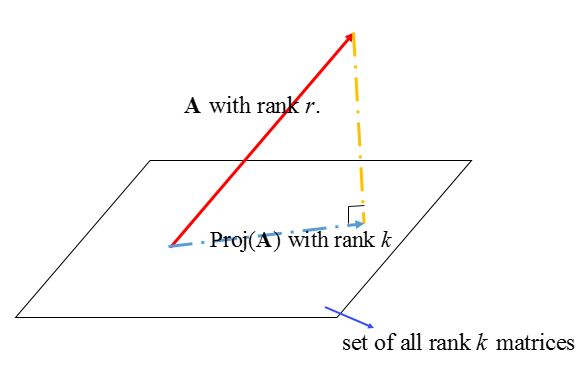
\includegraphics{week7/rank_r}
\caption{Best rank $k$ approximation: find the projection from matrix $\bm A$ with rank $r$ onto the plane that contains all rank $k$ matrices}
\end{figure}
\begin{remark}
Similarly, for the best rank $k$ approximation problem
\begin{align*}
  \min_{\bm Z}\quad        & \|\bm A-\bm Z\|^2_{F} \\
  \text{s.t.\quad} &  \rank(\bm Z)=k &     \\
                   &\bm Z\in\mathbb{R}^{m\x n}
\end{align*}
with $\bm A\in\mathbb{R}^{m\times n}$, the key is to do the projection of $\bm A$ onto the set $\mathcal{M}=\{\bm M \in\mathbb{R}^{m\times n}\mid \rank(\bm M)=k\}$, thus it suffices to solve the \emph{equality}
\[
\bm{Z}=\Proj_{\mathcal{M}}(\bm A).
\]
For some non-convex optimization problems, this idea is very useful. The further reading is recommended:
\begin{quotation}
Jain, Prateek, and P. Kar. "Non-convex Optimization for Machine Learning." Foundations $\&$ Trends® in Machine Learning 10.3-4(2017):142-336.
\end{quotation}
\end{remark}